\def\answers{257}

\subsection{Questionario}

Questa sezione riassume i risultati che abbiamo ricevuto dalle risposte al \href{https://docs.google.com/forms/d/1vKzFGCQb5nvyG6it8HfEqZgZ3ioQ6J1_T6eUiTdYIRc/edit}{questionario}. 
Prima di condividere il questionario, abbiamo effettuato un test \textbf{pilota} con 5 utenti per assicurarci che non ci fossero problemi o parti ambigue. Il numero finale di risposte ricevute al questionario è pari a \textbf{\answers}.

\subsubsection{Risultati}
Ai fini del questionario abbiamo raccolto informazioni statistiche, in particolare età e attuale posizione lavorativa. Dai risultati, il \textbf{45\%} è risultato essere studente, il \textbf{34\%} lavoratore, il \textbf{12\%} è studente-lavoratore e il rimanente è disoccupato. Per quanto riguarda l'età, il \textbf{53\%} ha tra i 18-25 anni, il \textbf{19\%} tra i 26 e i 35, l'\textbf{8\%} è minorenne e il restante \textbf{20\%} ha un'età superiore ai 50 anni.

\paragraph{}
Abbiamo scoperto che la metà degli intervistati visita i musei almeno una volta all'anno, mentre solamente in 4 hanno detto di visitarne almeno uno alla settimana.\\
Le visite guidate, dalle risposte, sembrano essere apprezzate e risultano essere utili. 
Si è scoperto che le persone preferiscono andare a visitare un museo in compagnia piuttosto che da soli, ma dalle risposte abbiamo capito che la maggior parte delle persone non trova interessante, o importante, ciò che i propri amici hanno visitato di recente, anche se allo stesso tempo hanno trovato molto utile la possibilità di organizzare visite di gruppo con essi attraverso l'utilizzo dell'applicazione.

\begin{figure}[ht]
    \centering
    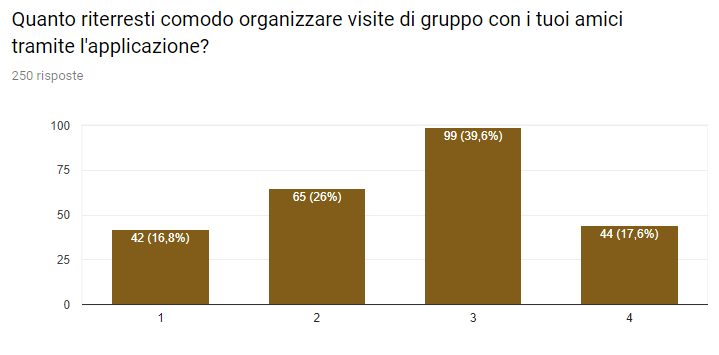
\includegraphics[width=1.0\textwidth]{images/charts-questionario/chart-visite-gruppo.png}
\end{figure}

\begin{figure}[ht]
    \centering
    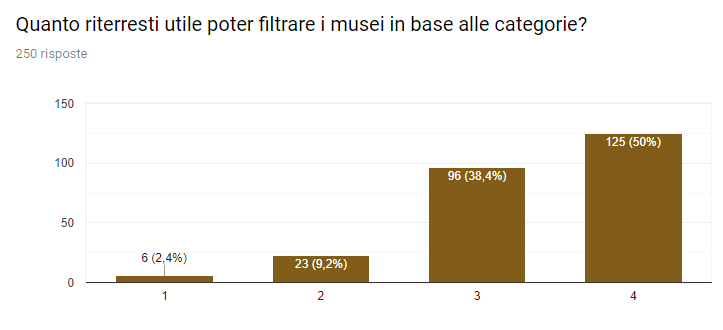
\includegraphics[width=1.0\textwidth]{images/charts-questionario/chart-filtro-categorie.png}
\end{figure}

\paragraph{}
La cosa davvero utile, a quanto pare, è la possibilità di filtrare i musei in base alle categorie che ci sono state segnalate nelle altre risposte.\\
Per quanto riguarda le recensioni, più dell'\textbf{80\%} ha detto di non rilasciarne dopo una visita, anche se comunque la scelta di visitare una mostra rispetto ad un'altra viene molto influenzata dalle recensioni della stessa. Infatti per il \textbf{54\%} delle persone le recensioni sono influenti, ma è importante che siano anche verificate, infatti il \textbf{77\%} ritiene utile poterne verificare l'attendibilità\\
Gli sconti di qualsiasi genere sembrano essere abbastanza utilizzati, a differenza delle visite gratuite.

\begin{figure}[ht]
    \centering
    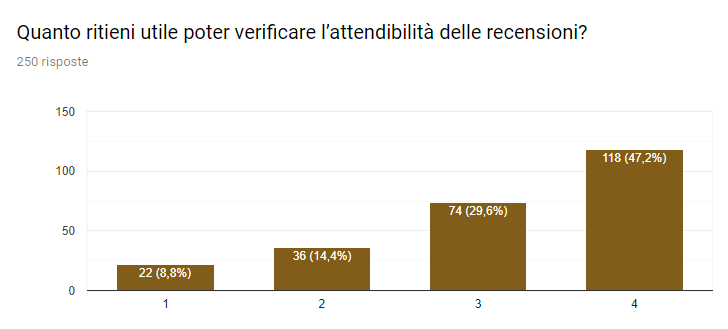
\includegraphics[width=1.0\textwidth]{images/charts-questionario/chart-verifica-recensioni.png}
\end{figure}